\documentclass{standalone}
\usepackage{graphicx}
\usepackage{tikz}
\usepackage{subfig}
\usepackage{float}
\usepackage{listings}
\usepackage{booktabs}
\usepackage{siunitx}
\usepackage{pgfplots}% Required for inserting images

%%% Configure pgf and tikz.
\pgfplotsset{compat=1.15}

\usetikzlibrary{arrows.meta}
\usetikzlibrary{3d, calc}
\definecolor{cyan}{HTML}{a6e6ff}
\definecolor{purple}{HTML}{A30262}
\definecolor{green}{HTML}{92e0ff}
\definecolor{Blue}{HTML}{091540}

\definecolor{QuanTEEMRed}{HTML}{F9123C}
\definecolor{QuanTEEMBlue}{HTML}{122D8D}
\definecolor{QuanTEEMOrange}{HTML}{FF6700}

%% Color package and configuration.
\usepackage{xcolor}

\begin{document}

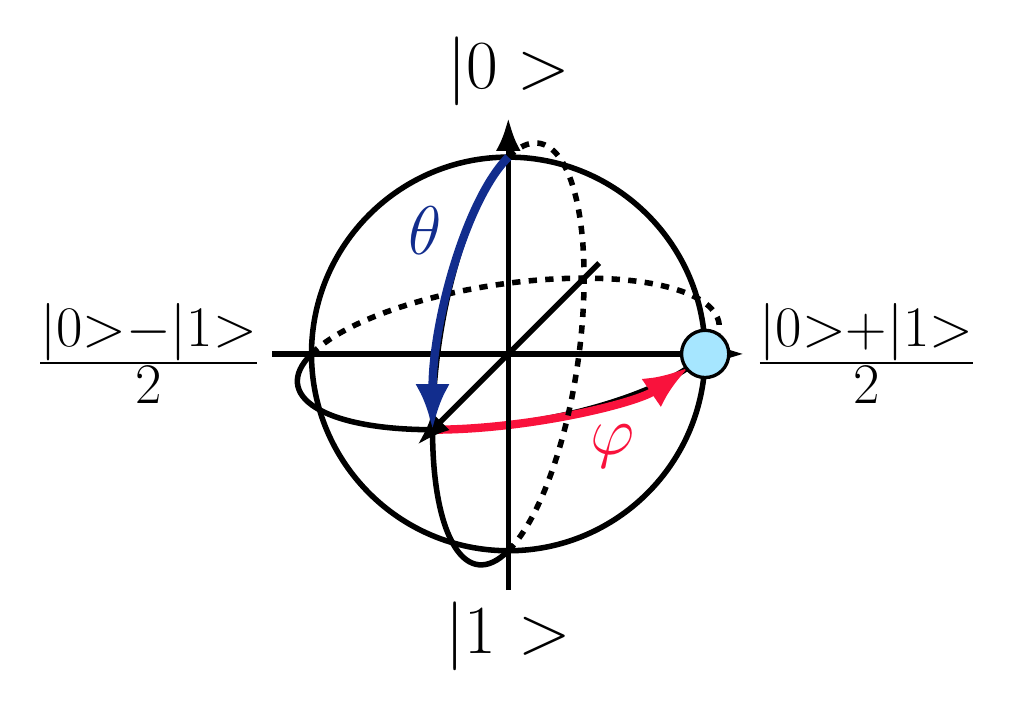
\begin{tikzpicture}

\begin{scope}[canvas is xy plane at z=0]
    \draw[line width=2] (0,0) circle (2.5);
\end{scope}

\begin{scope}[canvas is xz plane at y=0]
    \draw[line width=2] (2.5, 0) arc (0:180:2.5);
    \draw[dashed, line width=2] (2.5, 0) arc (0:-180:2.5);
    \draw[-Latex, line width=2] (-3, 0)
    node[left] {\Huge \bf $\frac{|0> - |1>}{2}$} -- (3,0)
    node[right] {\Huge \bf $\frac{|0> + |1>}{2}$};

    \draw[-Latex, line width=3, QuanTEEMRed] (0, 2.5) arc (90:10:2.5) node [midway, below right] {\Huge \bf $\varphi$};
\end{scope}


\begin{scope}[canvas is zy plane at x=0]
    \draw[line width=2] (0, 2.5) arc (90:-90:2.5);
    \draw[line width=2, dashed] (0, 2.5) arc (90:270:2.5);
    \draw[-Latex, line width=2] (0, -3) node[below]
    {\Huge \bf $\left|1\right.>$} -- (0, 3)
    node[above] {\Huge \bf $|0>$};

    \draw[-Latex, line width=2] (-3,0) -- (3,0);

    \draw[-Latex, line width=3, QuanTEEMBlue] (0, 2.5) arc (90:0:2.5) node [midway, above left] {\Huge $\theta$};
\end{scope}



% \draw [black, fill=cyan, very thick] (0, 2.5, 0) circle (0.3);

% \draw [black, fill=cyan, very thick] (0, 0, 2.5) circle (0.3);

\draw [black, fill=cyan, very thick] (2.5, 0, 0) circle (0.3);

\end{tikzpicture}
\end{document}
